\documentclass{article}


\usepackage{lmodern}
\usepackage[T1]{fontenc}
\usepackage[spanish,activeacute]{babel}
\usepackage[utf8]{inputenc}
\usepackage{mathtools}
\usepackage[colorlinks=true]{hyperref}
\usepackage{url}
\hypersetup{
    colorlinks=true,
    linkcolor=blue,
    filecolor=magenta,      
    urlcolor=cyan,
}
\usepackage{graphicx}
\graphicspath{ {latex/figures_tests/pdf/skern/} }
\title{TFG}
\author{Jorge Marco Esteve}

\begin{document}
\maketitle

\section{Antecedentes}
\subsection{Optical Music Recognition (OMR)}

 Estos últimos años, la disponibilidad de grandes colecciones de partituras digitales ha facilitado tanto la práctica
profesional de la musica como el acceso del aficionado a fuentes impresas que eran difíciles de obtener en el pasado.
Podemos encontrar ejemplos de estas colecciones en diferentes páginas web que llegan a almacenar cientos de miles de partituras
como es el caso de IMSLP. Además, las bibliotecas públicas y privadas realizan muchos esfuerzos para publicar sus coleciones
online como es en el caso de \url{https://drm.ccarh.org}. Sin embargo, a demás de esta accesibilidad a contenido musical, las
ventajas de tener una imagen digitalizada de cualquier obra no se limita a la facilidad de copiarlas y distribuirlas, dichas obras 
digitalizadas ofrecen una ausencia de desgaste que el recurso físico no es capaz de ofrecer.

Las grandes posibilidades que las aplicaciones actuales basadas en música pueden ofrecer están restringidas a partituras codificadas
simbólicamente. El problema de este método es que la transcripción de las partituras se realiza de forma manual. Al hacerse de esta
forma, el costo, tanto en tiempo como en recursos, es prohibitivo. Para paliar este inconveniente sería necesario recurrir a un sistema
 de transcripción automática. El llamado Optical Music Recognition (OMR) se define como la investigación sobre cómo enseñar a las
computadoras a leer notación musical, con el fin de poder exportar su contenido al formato deseado de manera automática, similar a la
utilidad de una caja negra. A pesar de las grandes ventajas que supone su desarrollo, en estos momentos, OMR está a mitad de camino de
ser totalmente confiable, ya que existen problemas de tareas sencillas que obstaculizan de manera importante OMR como la eliminación de
las líneas del pentagrama, la localización y clasificación de símbolos, o el ensamblaje de notación musical. Sin embargo, los recientes
avances del aprendizaje automático y, específicamente, del aprendizaje profundo, no solo permite resolver estas tareas con facilidad,
sino también replantearlas para enfrentar todo el proceso de una manera más elegante y compacta, evitando ciertas reglas que hacen que los
sistemas se limiten al tipo de entradas al que estan diseñados.

Una cosa que cabe señalar y que resulta fundamental en este trabajo es que OMR trabaja bajo una representación agnóstica en la que
únicamente se tiene en cuenta el punto de vista gráfico a la hora de transcribir las partituras. Este trabajo intenta mejorar esta
inteligencia artificial (OMR) por medio de una representación semántica, la cual, codifica los símbolos de acuerdo con su significado
musical. Aqui entra en uso la gramática que se va a realizar en este trabajo: Kern y Mens, dado una notación moderna o mensural respectivamente.

\subsection{Kern y Mens}
 Actualmente hay varios sistemas de representación musical como puede ser DARMS, SCORE, EsAC, Kern, etcétera. Estos sistemas
de representación han sido usados para simbolizar partituras, ya sea para codificarlas a PDF y obtener escritos de ellas, o para
reproducirlas, obteniendo de dichos símbolos una melodía.

Humdrums ha diseñado una representación secuencial musical de manera vertical. En el que cada columna representa una voz de cada melodia
con el fin de representar finalmente una partitura. Esta representación vertical se denomina Kern, la cual, soporta notaciones trandicional del Oeste,
también denominada notación moderna y en ella podemos manipular:

    El tono: accidentes, claves, posición de claves, armadura, formula de compás...
    La duración: silencios, puntos, ligaduras, ligados...
    Articulaciones y Ornamentos: staccato, tenuto, pizzicato...

Ademas de otros aspectos que podemos manipular en este tipo de representación.

 Una variante de la representación de Kern es Mens. Este tipo de representación acoje todo tipo de notación mensural blanca
con muchas coincidencias con Kern a la hora de representarse, ya que este tipo de notación también es vertical y se gestiona
de una forma muy parecida a la de notación moderna.

El defecto que lleva a esta representación a no estar realmente completa es la falta de gramática que es el tema correspondiente
a este trabajo.

\subsection{Gramática}
    Como diría el diccionario, gramática es un conjunto de normas y reglas que se usan para hablar y escribir correctamente una lengua.
La finalidad de este trabajo es crear una gramática lo mayormente competente como para poder, a partir de dichas normas y reglas, representar
cualquier tipo de notación musical de la manera más correcta posible. En este caso, la notación Kern y Mens será la adecuada para la creación
de la gramática.
    Obteniendo la primera gramática que comprende los dos tipos de notación: moderna y mensural.

Para implementar nuestra gramática utilizaremos un analizador sintáctico el cual va obteniendo tokens con la finalidad de
decidir si un conjunto de estos tokens cumplen las leyes de nuestra gramática. Hay dos tipos de analizadores sintacticos:
analizador sintáctico descendente y analizador sintáctico ascendente. El primero parte de una regla inicial y concluye en unos
tokens que son generados por las reglas. Mientras el analizador sintactico ascendente parte de un determinado grupo de tokens con
el fin de llegar a una regla principal.

Nosotros utilizaremos un analizador sintáctico descendente ya que dada la complejidad que nos puede suponer una gramática musical,
uno de las cosas positivas del analizador sintáctico descendente respecto al ascendente es, además de su eficiencia, su sencillez a
la hora de implementarlo.

Para implmentar nuestro analizador usaremos una herramienta denominada ANTLR4. Con esta herramienta podemos contruir reconocedores
, intérpretes, compiladores y traductores de lenguajes a partir de descripciones gramaticales de los mismos.

\section{Banco de ejemplos}
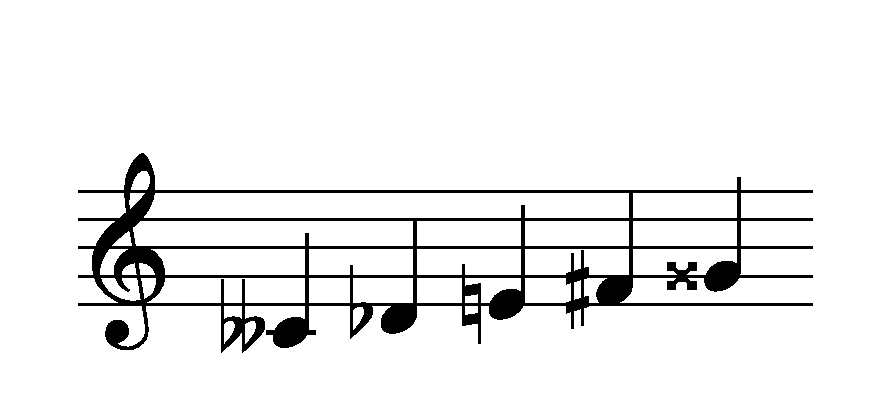
\includegraphics{accident1.pdf}
\end{document}